%----------------------------------------------------------------------------------------
% Requisiti
%----------------------------------------------------------------------------------------

\documentclass[10pt]{softeng} % Document font size and equations flushed left

%----------------------------------------------------------------------------------------
%	DOCUMENT INFORMATION
%----------------------------------------------------------------------------------------

\Phase{Inception - I iterazione}

\DocumentTitle{Requisiti di progetto} % Document title

%----------------------------------------------------------------------------------------

\begin{document}

\startofdocument{}

\section{Definizione dei requisiti}

Si vuole realizzare un sistema di Home Banking (da ora HBS) per la gestione di fondi privati a breve, medio e lungo termine via Web. Il sistema è rivolto a Banche che decidono di implementare il protocollo/software Open Bank Project. Si presuppone che la banca già abbia uno stabile ed efficiente sistema di database di proprietà con opportuni software accessori, e in generale non si vuole analizzare la parte relativa al back-end della banca.  

%TODO la scelta è stata fatta non nel documento di fattibilit\`a ma nella proposta di progetto
Per rispettare e meglio implementare alcuni fondamentali requisiti non funzionali (sicurezza, tempi di reazione del sistema, ecc.), durante la stesura del documento di fattibilità si è deciso di rimanere nell'ambito del \emph{retail banking}, ossia di progettare un sistema i cui unici utenti siano persone fisiche e non imprese o altri istituti finanziari.

Ogni individuo iscritto ad una banca possiede almeno un conto su cui depositare i propri risparmi: può essere \emph{di deposito} o \emph{corrente} a seconda che siano permesse le sole operazioni di prelievo e deposito o che in aggiunta a queste sia possibile  effettuare bonifici, pagamento di assegni, prelievi bancomat e simili.

\subsection{Utenti del sistema}

Gli utenti di questo sistema si dividono principalmente in due categorie: utenti registrati, o correntisti, e dipendenti della banca. 

Un individuo può ottenere un \emph{account HBS} in due passi:
\begin{enumerate}
	\item
	\begin{enumerate}
		\item se è già correntista della banca, gli basta fornire ad un dipendente della banca il proprio numero di conto;
		\item se non è correntista, deve compilare i moduli necessari all'apertura di un conto corrente (on-line o presso una filiale);
	\end{enumerate}
	\item in ogni caso, l'individuo deve recarsi in una filiale per consegnare copia di documento d'identità e ricevere le 					\emph{credenziali d'accesso} del proprio account.
\end{enumerate}

Ad ogni account HBS è associato, oltre al conto corrente, un portafoglio azionario per conservare tutti i titoli bancari di cui il correntista sia in possesso. Un portafoglio azionario ha un valore, calcolato in funzione dei valori di ogni azione contenuta al suo interno: modifiche di questo valore influiscono sul conto corrente associato al portafoglio, e il correntista non solo deve poter visionare tale valore e il suo andamento nel tempo, ma deve anche poter gestire il contenuto del portafoglio stesso.

%TODO ?e se un correntista vuole aprire un altro conto?

%TODO usare termini positivi (non "minimale")
Le funzionalità che verranno descritte per gli \emph{account di servizio} e per gli \emph{account HBS} sono un  nucleo minimale, o \emph{kernel}, ritenuto ``necessario'' per assolvere ai compiti essenziali di un qualsiasi sistema di home banking.
Il \emph{pool} di progettisti e sviluppatori si impegna a implementare questo kernel nel modo più riutilizzabile e scalabile possibile, in modo da lasciare alla banca che adotti questo sistema la possibilità di operare come meglio crede con queste funzionalità, ad esempio creandone altre a partire da quelle qui elencate.

Un correntista deve poter:
\begin{itemize} 
	\item visionare \emph{saldo contabile annuale}, relativo all'anno in corso con eventuali grafici Valore/Tempo dell'andamento del valore rispetto agli anni precedenti;
	\item visionare \emph{saldo contabile mensile}, relativo al mese corrente con eventuali grafici Valore/Tempo dell'andamento del valore rispetto ai mesi precedenti;
	\item visionare \emph{saldo liquido} relativo al giorno corrente , nel caso in cui voglia compiere operazioni bancarie che coinvolgano calcolo di \emph{interesse};
	\item visionare \emph{saldo disponibile}, relativo al giorno corrente;
	\item visionare uno storico delle transazioni effettuate, avendo a disposizione per ogni transizione la \emph{data contabile}, l'\emph{importo versato} ed una \emph{causale};
	\item poter annullare una transazione ancora non completata confermata;
	\item visionare informazioni delle carte di credito eventualmente collegate al conto;
	\item effettuare operazioni ``veloci'', ossia inserire pochi dati in una maschera preconfigurata e confermare l'operazione mediante meccanismo TOTP:
	\begin{itemize}
			\item ricariche telefoniche;
%			\item bonifici ordinari e bonifici SEPA mediante compilazione di opportuni moduli on-line;
			\item pagamento delle bollette;
	\end{itemize}
	\item visionare l'andamento in borsa dei titoli azionari del suo portafoglio;
	\item vendere uno o più titoli azionari del proprio portafoglio;
	\item investire il proprio patrimonio nei titoli di credito statali (NON azionari) a medio e lungo termine che ritiene più opportuni, avendo a disposizione un \emph{benchmark} per valutarne l'andamento in borsa e il profilo di rischio;
\end{itemize}	

I dipendenti della banca si dividono in \emph{impiegati} e \emph{dirigenti}. A ogni dipendente, sia esso impiegato o dirigente, viene assegnato un \emph{account HBS di servizio}, con cui egli può assolvere alle sue mansioni specifiche; i vari account di servizio differiscono per permessi di accesso e funzionalità disponibili.

Ad ogni \emph{account di servizio} sono assegnati:
\begin{itemize}
	\item i dati anagrafici del relativo dipendente;
	\item una password ``speciale'' (decidere politica di sicurezza).
\end{itemize}	

Gli \emph{impiegati}, mediante il loro account di servizio, devono poter: 
\begin{itemize}
	\item confermare/respingere atti che richiedono esplicita approvazione, ad esempio i bid per conti o carte inviati dagli utenti; 
	\item effettuare eventuali operazioni minori di contabilità che una banca potrebbe permettere via internet
\end{itemize}

I \emph{dirigenti} devono poter:
\begin{itemize}
	\item accedere e modificare i disclaimer pubblicitari del sito di home banking;
	\item impostare e modificare opportuni pacchetti di azioni o di fondi d'investimento e in generale offerte che si vogliono propinare agli utenti;
	\item selezionare, mediante opportuna combinazione di \emph{queries}, categorie o fasce di utenti in base a diversi parametri socio-economici, ed ottenere precise statistiche al riguardo.
	\item confermare atti di importanza ``superiore'' (a.e. alti investimenti in titoli azionari, transazioni di danaro molto elevate da un conto corrente ad un altro, ecc.), in seguito all'approvazione iniziale di un impiegato.
\end{itemize}

\subsection{Transazioni}

Una transazione economica è il passaggio sicuro e irreversibile da un conto ad un altro di una certa quantità di denaro.
La somma viene accreditata al \emph{conto destinatario} e detratta al \emph{conto mittente}, indipendentemente dalle banche di appartenenza, sfruttando ``indirizzi bancari'' come il codice IBAN.

%TODO cambiare in "bonifici programmati"

%Il nostro sistema vuole dare la possibilità alla banca che lo implementi di adottare una politica di ``conferma della transazione'': in uno scenario di e-commerce, una transazione tra un certo \emph{mittente} e un certo \emph{destinatario} viene confermata se il primo conferma di aver ricevuto in modo corretto il bene acquistato dal secondo, annullata se, viceversa, il primo è in grado di dimostrare la non corretta o avvenuta ricezione del bene acquistato.
%Per permettere questa funzionalità, si suddividerà la procedura di pagamento on-line in più step, ognuna delle quali avrà determinate peculiarità.

\subsection{Titoli di credito}

I titoli di credito sono, generalmente, strumenti finanziari mediante i quali i correntisti investono il proprio danaro: possono essere fondi comuni di investimento o azioni.
Ogni titolo di credito deve avere un \emph{benchmark}, calcolato dalla banca e visibile all'utente, che ne specifichi la \emph{volatilità} sul mercato.
Per motivi di sicurezza ed efficienza del sistema, si decide di non permettere l'acquisto diretto di titoli di credito su mercato nazionale e internazionale, ma di lasciare ad un account utente la possibilità di acquisire pacchetti preconfezionati dalla banca stessa.
Tuttavia ogni correntista può, attraverso il proprio account, avere delle dettagliate informazioni sull'andamento in borsa dei titoli che conserva nel suo portafoglio  e gli è lasciata la possibilità di vendere tali titoli nel caso lo ritenga opportuno.

\subsection{Bidding}

\`E possibile per un correntista o un individuo non registrato \emph{fare bidding}, ossia richiedere alla banca l'apertura di un conto corrente o il rilascio di una carta di credito con determinate condizioni.
In base a delle regole definite dai dirigenti questa proposta pu\`o essere:
\begin{itemize}
	\item approvata automaticamente dal sistema;
	\item inoltrata a un dipendente della banca per l'approvazione;
	\item rifiutata automaticamente.
\end{itemize}

Un possibile sistema di regole per l'approvazione dei bidding \`e l'individuazione di \emph{aree di risposta} basate sui parametri personalizzabili, come costo mensile di una carta di credito, tetto di spesa massima mensile, capacit\`a di prelievo allo sportello, etc.
Un esempio di come identificare queste aree di risposta \`e dato in figura \ref{fig:bidding}:
\begin{itemize}
	\item la zona compresa fra le linee tratteggiate verdi indica le condizioni (in questo caso una coppia di valori ``spesa massima mensile'' e ``costo mensile'' per una carta di credito) approvate automaticamente;
	\item la zona compresa fra le linee tratteggiate arancioni indica le condizioni soggette a verifica del dirigente della filiale prima dell'accettazione o del rifiuto;
	\item la zona compresa fra le linee tratteggiate rosse indica le condizioni rifiutate automaticamente.
		Le motivazioni di un rifiuto automatico possono essere differenti: un tetto di spesa mensile troppo alto a fronte di un costo mensile troppo basso potrebbe essere economicamente svantaggioso per la banca, mentre un tetto di spesa basso associato a un costo mensile alto potrebbe portare la banca a violare le normative vigenti a tutela dei suoi clienti.
\end{itemize}

\begin{figure}
	\resizebox{\columnwidth}{!}{
	\begin{tikzpicture}
		\begin{axis}[
			ymin=1,
			scale only axis,
			width=\columnwidth,
			ticks=none,
			domain=0:10,
			xlabel={Spesa massima mensile},
			ylabel={Costo mensile},
			axis lines=left,
			samples=200
        ]
		    \path[name path=axis] (axis cs:0,0) -- (axis cs:1,0);
		    \addplot[green] {x};
		    \addplot[green, dashed] {x-1};
		    \addplot[green, dashed] {x+1};
		    \addplot[orange, dashed] {x-2};
		    \addplot[orange, dashed] {x+2};
		    \addplot[red, dashed] {x-3};
		    \addplot[red, dashed] {x+3};
%   			\node [] at (axis cs:0.2,0) {basso};
%   			\node [] at (axis cs:0.6,0.3) {medio};
%   			\node [] at (axis cs:1.0,0.6) {alto};
%   			\node [] at (axis cs:1.4,1.2) {massimo};			
		\end{axis}
	\end{tikzpicture}
	}
	\caption{Un esempio di bidding: confronto fra spesa massima mensile di una carta di credito e costo di mantenimento della stessa.}
	\label{fig:bidding}
\end{figure}

Il sistema di bidding pu\`o portare diversi vantaggi alla banca che lo adotti:
\begin{itemize}
	\item fidelizzazione dell'utenza: un simile meccanismo permette alla banca di venire incontro alle esigenze di clienti di lunga data o con alta giacenza media mensile, che risultano essere ``buoni'' secondo le metriche della dirigenza, fornendo una possibilit\`a di interazione maggiore all'utente;
	\item contrasto della concorrenza: un cliente della banca potrebbe ricevere un'offerta conveniente da un istituto concorrente, ma scoprire autonomamente che un'offerta simile \`e disponibile anche presso la sua banca attuale;
	\item riduzione delle spese: automatizzando parte della ricerca dei contratti si riduce il carico di lavoro che i dipendenti della banca devono subire.
\end{itemize}

Un sistema di bidding presenta dei rischi, fra cui:
\begin{itemize}
	\item il sistema per stabilire i parametri di accettazione automatica potrebbe essere poco intuitivo e non fornire le metriche giuste, e il dirigente che se ne occupa viene portato a scelte che vanno contro gli interessi del suo istituto;
	\item il sistema di bidding potrebbe essere troppo complesso per l'utenza della banca e non venir utilizzato.
\end{itemize}
Tutti questi rischi devono essere gestiti correttamente durante lo sviluppo del sistema.

%TODO pubblicità contestuale on-demand di bidding?




\section{Specifica dei requisiti}

Di seguito \`e illustrata la specifica dettagliata dei requisiti.

\subsection{Requisiti funzionali}

\emph{Da determinare}

\subsection{Requisiti non funzionali}

\emph{Da determinare}

\subsubsection{Requisiti di sicurezza del sistema}
 
Le credenziali d'accesso sono per un account sono:
\begin{itemize}
	\item dati anagrafici del correntista;
	\item numero conto corrente;
	\item password scelta dal correntista.
\end{itemize}
	
Una volta che ha effettuato l'accesso,  l'utente deve poter svolgere le seguenti operazioni senza fornire la One Time Password:
\begin{itemize}
	\item Visionare saldo contabile, disponibile e liquido.
	\item Visionare uno storico delle transazioni effettuate.
	\item Visionare informazioni riguardo le carte di credito collegate al conto (se presenti).
	\item Effettuare ``operazioni veloci'' impostate attraverso un sistema di configurazione.
\end{itemize}

Invece è necessario fornire la One Time Password per:
\begin{itemize}
	\item effettuare transazioni, come:
	\begin{itemize}
		\item bonifici ordinari e bonifici SEPA;
		\item ricariche carte prepatate e schede telefoniche;
		\item pagamento bollette, bollettini, tasse, etc;
	\end{itemize}
	\item configurare operazioni veloci;
	\item ogni altra operazione sensibile.
\end{itemize}

Ogni operazione effettuata da un utente sul sistema deve essere registrata in un log.
In particolare, ogni log deve contenere almeno:
\begin{itemize}
	\item l'operazione eseguita;
	\item il conto coinvolto nell'operazione;
		%TODO rivedere codesta parte: codice univoco della transazione al posto del conto?
		% analizzare bene come funziona OBP
	\item l'istante dell'operazione;
	\item informazioni riguardanti il terminale da cui \`e stata effettuata l'operazione.
\end{itemize}

\subsection{Requisiti di dominio}

La legislazione attuale richiede che gli organi di controllo finanziario come la Banca d'Italia e le forze dell'ordine possano accedere in lettura a tutte le informazioni salvate dal sistema di Online Banking.

Ogni sistema informatico nell'ambito bancario deve permettere l'accesso da remoto alla sua rete interna tramite il meccanismo di \emph{VPN}.
%TODO glossario vpn - virtual private network.
Fornire alle autorit\`a di controllo le credenziali e/o interfacce per accedere ai sistemi di \emph{data storage}.

In particolare le forze dell'ordine devono poter:
\begin{itemize}
    \item Dato un utente visualizzare le seguenti informazioni:
        \begin{itemize}
            \item Tutte le transazioni effettuati dall'utente.
            \item Tutte le transazioni che hanno l'utente come destinatario.
            \item Dati anagrafici dell'utente.
            \item Informazioni riguardo al terminale informatico dal quale l'\emph{account} dell'utente \`e stato acceduto in precedenza.
        \end{itemize}
    \item In caso le informazioni siano ridondanti il sistema pu\`o fornire alle ff. oo. un modo per confrontare le informazioni e fare il controllo di coerenza.
\end{itemize}
        %TODO da qualche parte bisogna dire che un haxxor in genere non puo modificare tutti i log in maniera coerente, perche pensa a rubare i dindi invece di giocare ad uplink

L'organo di controllo finanziario deve poter:
\begin{itemize}
    \item Dato un utente visualizzare le seguenti informazioni:
        \begin{itemize}
            \item Tutte le transazioni effettuati dall'utente.
            \item Tutte le transazioni che hanno l'utente come destinatario.
            \item Lo storico di Online Trading dell'utente.
        \end{itemize}
    \item Visualizzare le informazioni dei pacchetti di Online Trading.
    \item Visualizzre lo storico del sistema di Online Trading.
    \item Visualizzare lo storico del sistema di Bidding.
    %non so se ci va visualizzare mutui e tassi
\end{itemize}






\section{Glossario}
%(versione 1 : sono omesse definizioni banali e/o implicite)

\paragraph{Audit di sicurezza} 
	operazioni di controllo del sistema effettuate periodicamente per controllare che non ci siano sate violazioni della politica di sicurezza adottata
\paragraph{Banca D'Italia}
	 Banca centrale della Repubblica Italiana, avente funzione sia di vigilanza su banche, istituti di credito, intermediari finanziari sia di principale controllore in materia di antiriciclaggio: insieme alla CONSOB, deve avere libero accesso, entro i termini previsti dalla legge, ai dati contenuti nei database di qualsiasi istituto finanziario che operi sul territorio italiano. \cite{banca_italia}
\paragraph{Bonifico}     
	operazione bancaria mediante la quale si mette a disposizione di una persona o le si accredita una somma di denaro per ordine e conto di altri
\paragraph{Bonifico Sepa}
	bonifico (v.bonifico) accreditabile ad un destinatario ubicato oltre i confini nazionali nell'area SEPA.
\paragraph{Conto Corrente (cc)}
	indica un deposito di danaro effettuato dal possesore del bene, detto \emph{correntista}, in una banca o istituto di credito
\paragraph{Codice IBAN}
	L'International Bank Account Number è uno standard internazionale utilizzato per identificare un'utenza bancaria e/o operazione associata ad un conto corrente 
\paragraph{Codice BIC/SWIFT}
	standard che definisce i \emph{bank identifier codes} (codici d'identificazione bancaria) approvato dall'International Organization for Standardization (ISO). Questi codici vengono utilizzati per i trasferimenti di denaro tra banche, specialmente nelle transazioni internazionali, per le quali è spesso ancora necessario nonostante l'entrata in vigore dell'IBAN. \cite{bic_wiki}
\paragraph{Commissione Nazionale per le societ\`a e la borsa (CONSOB)}
	è un'autorità amministrativa indipendente, dotata di personalità giuridica e piena autonomia la cui attività è rivolta alla tutela degli investitori, all'efficienza, alla trasparenza e allo sviluppo del mercato mobiliare italiano. \cite{consob_wiki}
\paragraph{Fondo comune di investimento}
	è un istituto d'intermediazione finanziaria mediante il quale è possibile partecipare, investita una determinata quota di danaro, alla gestione e alla spartizione di dividendi prodotti da un determinato \emph{bene mobiliare} nel tempo. La \emph{banca depositaria} ne custodisce materialmente i titoli e ne tiene in cassa le disponibilità liquide. Le banche hanno inoltre un ruolo di controllo sulla legittimità delle attività del fondo sulla base di quanto prescritto dalle norme della Banca d'Italia e dal regolamento del fondo stesso
\paragraph{Istituto di credito}
	organismo che svolge simultaneamente l’attività di raccolta di risorse finanziarie e di concessione del credito per proprio contoa terzi 
\paragraph{Open Bank Project (OBP)}
	è una API open source che permette a banche ed istituti di credito di creare un interfaccia utente di ampia portata e fruibilità. Essendo un sistema molto versatile e largamente riadattabile, si presta molto a definire un vero e proprio \emph{standard di interfaccia}, ossia a definire un canone per la creazione di interfacce rivolte e all'utenza bancaria generica e agli organismi deputati al controllo bancario. \cite{obp}
\paragraph{Portafoglio valori/titoli azionari}
	è l'insieme dei diversi titoli finanziari e/o fondi d'investimento che l'utente bancario generico può possedere.Ogni titolo e/o fondo acquisito viene inserito nel portafoglio.
\paragraph{Refactoring}
	processo di riutilizzazzione di codice già scritto in precedenza, senza doverne generare di nuovo
\paragraph{SEPA}
	La SEPA (Single Euro Payments Area) è l’area unica in cui i cittadini, le imprese e gli enti, possono eseguire e ricevere pagamenti in Euro, all’interno dei confini nazionali e tra i paesi diversi che compongono l’area SEPA con condizioni di base, diritti ed obblighi uniformi tra i paesi stessi. 
\paragraph{Time-based One Time Password (TOTP)}
	è un algoritmo che calcola una \emph{One-Time password} combinando mediante una funzione hash una chiave segreta condivisa ed il tempo corrente. \cite{totprfc}
\paragraph{Trading online}
	pratica uguale a quella del \emph{trading} bancario classico mediante aiuto di personalità con competenze specifiche(v.broker), effettuata però in rete, disponendo cioè di opportuni strumenti software per il monitoraggio di mercati azionari nazionali e internazionali e  per il controllo completo e \emph{real time} del proprio portafoglio azionario.


\section{Business cases}

Di seguito sono i business case individuati a partire dalla definizione dei requisiti e dall'analisi del contesto:
\begin{itemize}
	\item Procedura di registrazione di un utente (figura \ref{fig:business_case_registration}).
	\item Procedura di autenticazione di un utente registrato (figura \ref{fig:business_case_authentication}).
	\item Procedura generica per effettuare un'operazione all'interno del sistema di Home Banking (figura \ref{fig:business_case_generic_operation}).
	\item Procedura generica di controllo da parte di un'entit\`a preposta (figura \ref{fig:business_case_control_activity}).
\end{itemize}
Nei business case utilizziamo la freccia tratteggiata (\emph{message flow}) fra gateway di \emph{pool} differenti per rappresentare sinteticamente il propagarsi dell'effetto di una decisione dalla coda alla testa della freccia.
Ad esempio, nella figura \ref{fig:business_case_authentication}, la validit\`a delle credenziali viene stabilita dal software di Home Banking, e la conclusione di questa decisione si ``riflette'' nel browser del cliente, che riceve una pagina di errore o una schermata di successo a seconda del risultato.

\section{Registro modifiche}

\subsection{Inception}

\subsubsection{I iterazione}

Prima stesura documento.

%Un utente registrato pu\`o ottenere una lista delle tipologie di servizi offerti dalla banca che pu\`o sottoscrivere.
%
%Un utente pu\`o aprire diversi tipi di conto corrente, 
%
%Un utente titolare di un conto.
%
%Audit di sicurezza:
%storico delle connessioni e delle operazioni riguardanti il conto corrente.
%
%Il sistema di home banking \`e personalizzabile dagli impiegati della banca.
%I dipendenti della banca possono creare:
%- conti di deposito
%- carte di credito/debito
%Personalizzando vari parametri.
%I dirigenti possono permettere l'apertura di certi conti/carte solo a clienti che abbiano i requisiti specificati:
%- giacenza media
%- capitale depositato che aumenta
%- boh
%
%Possibilit\`a di bidding in cui un utente fa una proposta alla banca per ottenere un conto o una carta con certe particolari condizioni/agevolazioni.
%In base a delle regole definite dai dirigenti questa proposta pu\`o essere:
%- approvata automaticamente dal sistema
%- inoltrata a un manager per l'approvazione
%- rifiutata automaticamente
%Controllare se la cosa \`e legale o se ce ne freghiamo.
%
%
%
%%--------------------------------------------------------------
%
%% TODO ripulire questa parte e spostare tutto nel file dei requisiti
%Per rafforzare i requisiti non funzionali (come i requisiti di sicurezza) si sceglie di rivolgere il sistema di Home Banking a persone fisiche (retail banking).
%
%Alcune delle funzionalit\`a che il sistema pu\`o offrire sono:
%\begin{enumerate}
%	\item L'utente si deve poter pre-registrare online fornendo i suoi dati anagrafici, e:
%		\begin{enumerate}
%			\item se l'utente ha gi\`a un conto aperto con la banca, pu\`o fornire il suo numero di conto;
%			\item se l'utente non ha gi\`a un conto con la banca, pu\`o scegliere diverse soluzioni con agevolazioni differenti e pre-compilare i moduli necessari all'apertura del conto.
%				% TODO: cambiare "se l'utente ha gi\`a un conto con la banca" in "se l'utente desidera aprire un nuovo conto"
%		\end{enumerate}
%		Un utente pre-registrato pu\`o recarsi presso una filiale della banca e ultimare la registrazione presentando il documento d'identit\`a.
%		La banca gli fornir\`a le informazioni per l'accesso.
%		Ai nuovi clienti viene fornito su richiesta un bancomat.
%		% TODO: rimuovere, non \`e di interesse per l'applicazione, facciamo home banking non ATM
%
%		Un utente non pre-registrato pu\`o effettuare la procedura completa di registrazione presso una filiale, fornendo le stesse informazioni richieste agli utenti che si pre-registrano online.
%	\item Le informazioni per l'accesso comprendono:
%		\begin{enumerate}
%			\item Il numero di conto;
%			\item La password del conto;
%			\item Un dispositivo TOTP\footnote{Time-Based One Time Password, RFC 6238. \url{https://tools.ietf.org/html/rfc6238}} per effettuare operazioni sensibili.
%		\end{enumerate}
%	\item Un utente registrato pu\`o effettuare il login al sistema di Home Banking fornendo le informazioni di accesso (requisito TOT), in particolare deve inserire numero di conto e password del conto.
%	\item Un utente che ha effettuato l'accesso al sistema di Home Banking deve poter svolgere le seguenti operazioni senza fornire la One Time Password:
%		\begin{enumerate}
%			\item Visionare saldo contabile, disponibile e liquido.
%			\item Visionare uno storico delle transazioni effettuate.
%			\item Visionare informazioni riguardo le carte di credito collegate al conto (se presenti).
%			\item Effettuare ``operazioni veloci'' impostate attraverso un sistema di configurazione (requisito TOT).
%		\end{enumerate}
%	\item Un utente che ha effettuato l'accesso al sistema di Home Banking deve poter effettuare le seguenti operazioni fornendo ogni volta la One Time Password:
%		\begin{enumerate}
%			\item Effettuare transazioni, come:
%				\begin{enumerate}
%					\item bonifici ordinari e bonifici SEPA;
%					\item ricariche carte prepatate e schede telefoniche;
%					\item pagamento bollette, bollettini, tasse, etc;
%				\end{enumerate}
%			\item Configurare operazioni veloci.
%			\item Se ci viene in mente altro ce lo mettiamo.
%		\end{enumerate}
%	\item Ogni operazione deve essere registrata in un log.
%		Devono essere mantenute le seguenti informazioni:
%		\begin{enumerate}
%			\item l'operazione eseguita;
%			\item il conto coinvolto nell'operazione;
%				% TODO rivedere codesta parte: codice univoco della transazione al posto del conto?
%				% analizzare bene come funziona OBP
%			\item l'istante dell'operazione;
%			\item informazioni riguardanti il terminale da cui \`e stata effettuata l'operazione.
%		\end{enumerate}
%	\item Il sistema deve poter essere configurabile dall'utente per inviare notifiche via SMS e/o via email a seguito di ogni evento stabilito dall'utente.
%		La banca pu\`o associare una tariffa per abilitare le notifiche su specifici insiemi di eventi.
%		Gli eventi notificabili possono includere:
%		\begin{enumerate}
%			\item Accesso al sistema;
%			\item Pagamento o prelievo dal conto;
%			\item Pagamento ricevuto.
%		\end{enumerate}
%\end{enumerate}

%----------------------------------------------------------------------------------------
%	REFERENCE LIST
%----------------------------------------------------------------------------------------

%\nocite{banca_italia}
\printcustombibsmall{}

%----------------------------------------------------------------------------------------
%	FIGURES
%----------------------------------------------------------------------------------------

%\begin{figure*}[hbt]
%	\centering
%	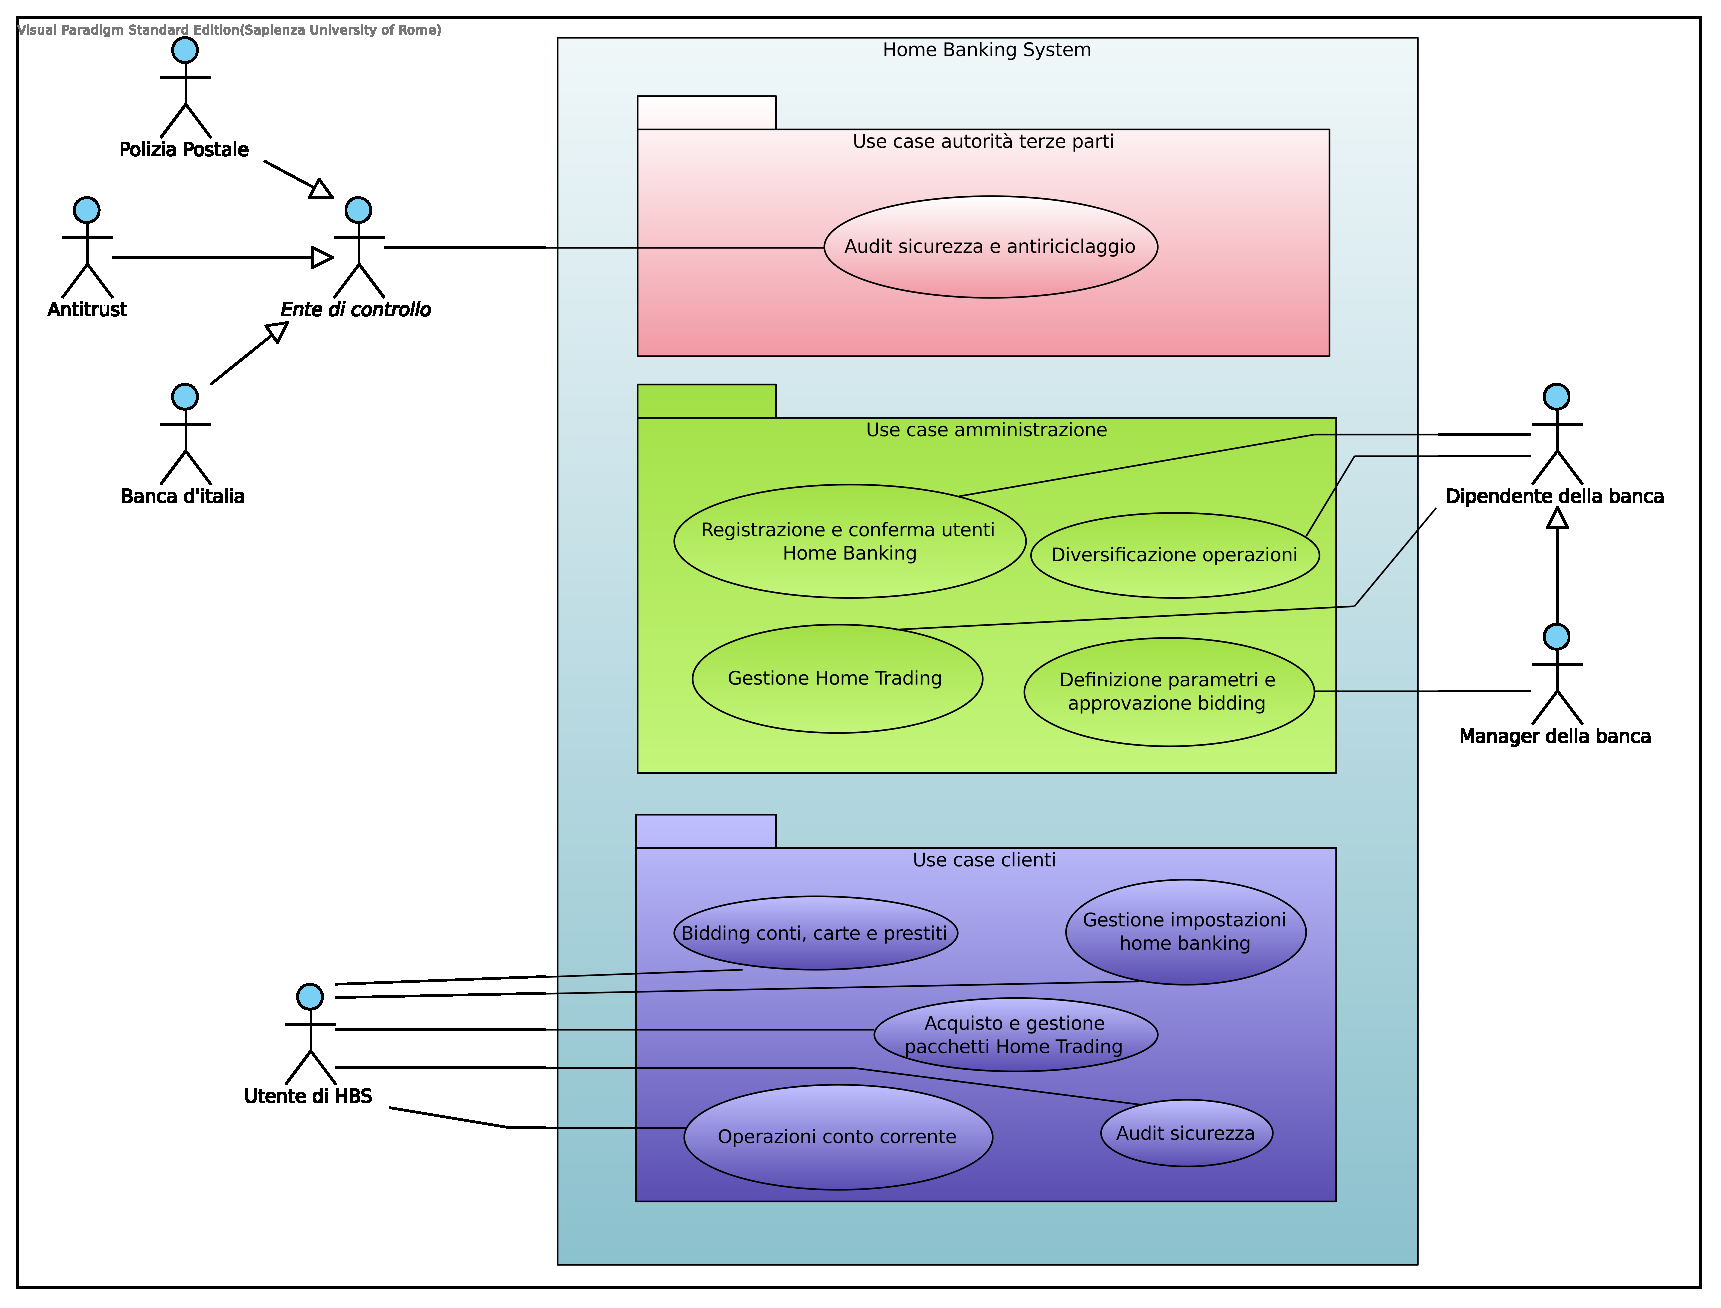
\includegraphics[width=\textwidth]{Images/Home_Banking_inception_use_cases.eps}
%	\caption{Attori del sistema di Home Banking e relativi use cases.}
%	\label{fig:inception_use_cases}
%\end{figure*}

\begin{figure*}[hbt]
	\centering
	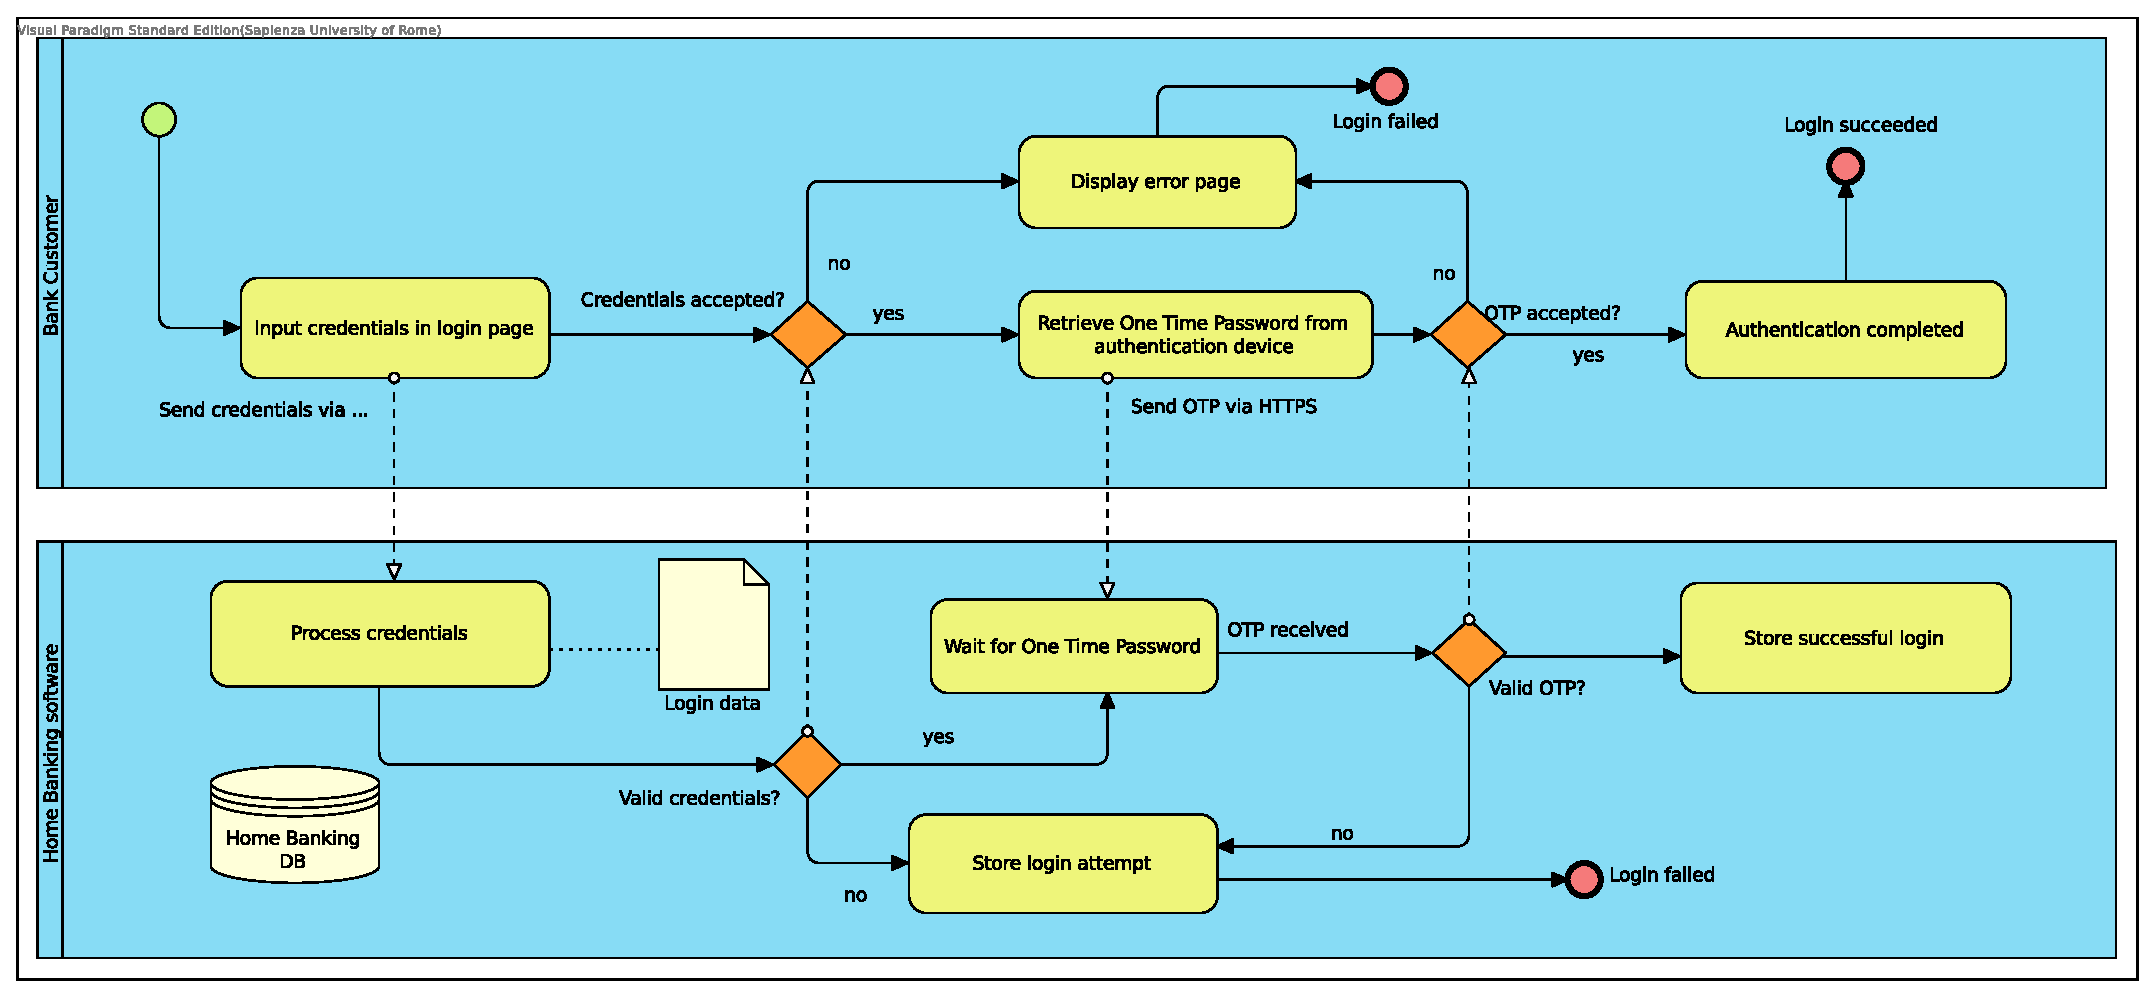
\includegraphics[width=\textheight, angle=90]{Images/Authentication.eps}
	\caption{Business case: procedura di autenticazione.}
	\label{fig:business_case_authentication}
\end{figure*}

\begin{figure*}[hbt]
	\centering
	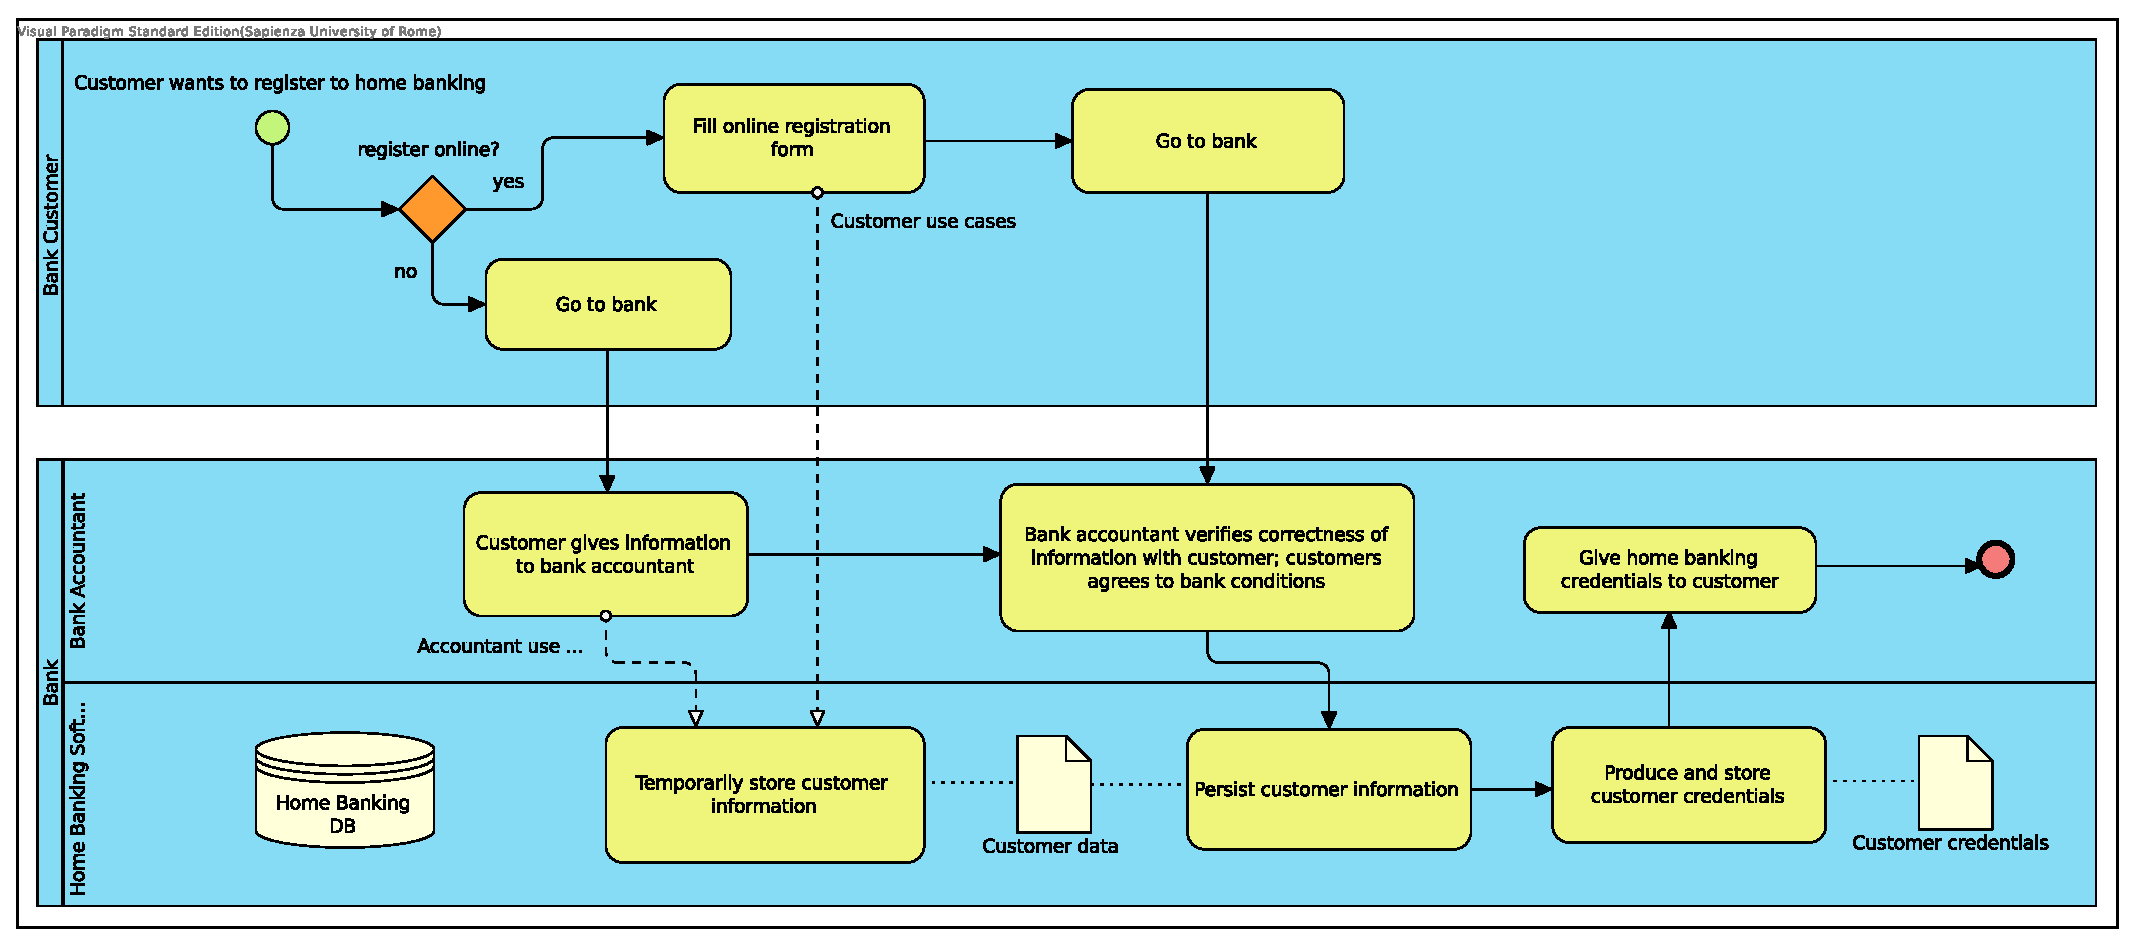
\includegraphics[width=\textheight, angle=90]{Images/Home_Banking_registration.eps}
	\caption{Business case: procedura di registrazione.}
	\label{fig:business_case_registration}
\end{figure*}

\begin{figure*}[hbt]
	\centering
	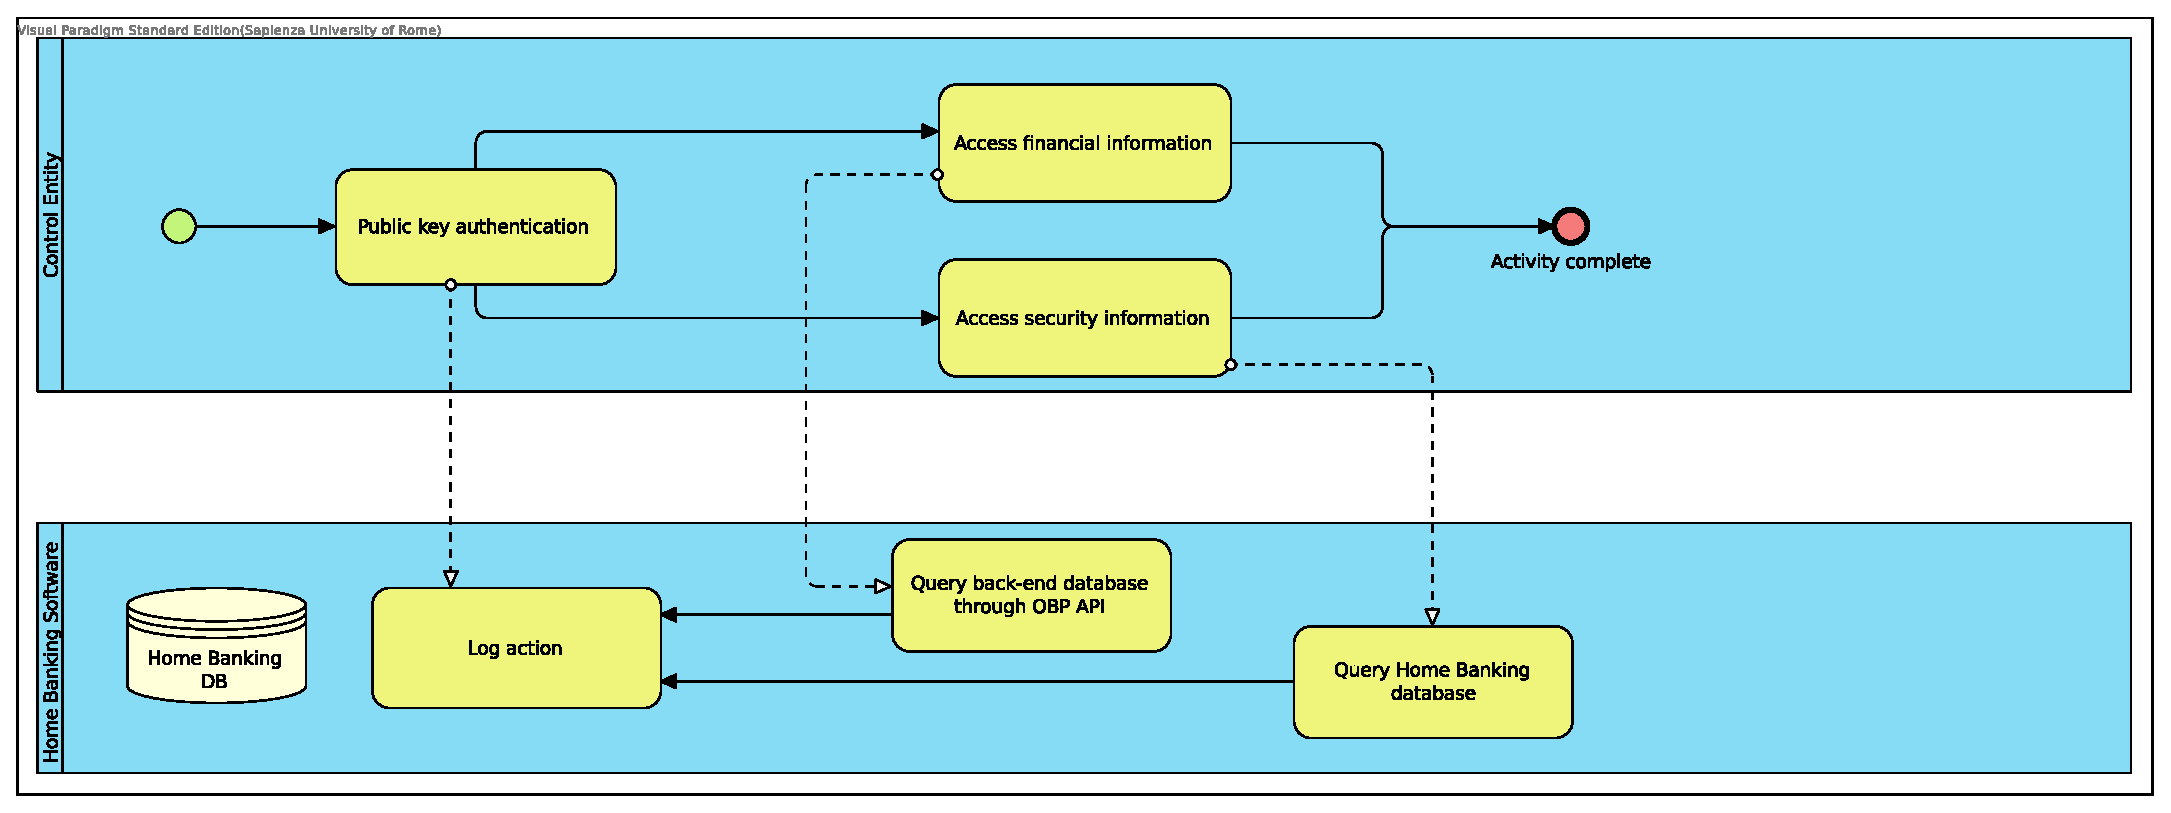
\includegraphics[width=\textheight, angle=90]{Images/Home_Banking_control_activity.eps}
	\caption{Business case: attivit\`a di controllo effettuata da enti responsabili.}
	\label{fig:business_case_control_activity}
\end{figure*}

\begin{figure*}[hbt]
	\centering
	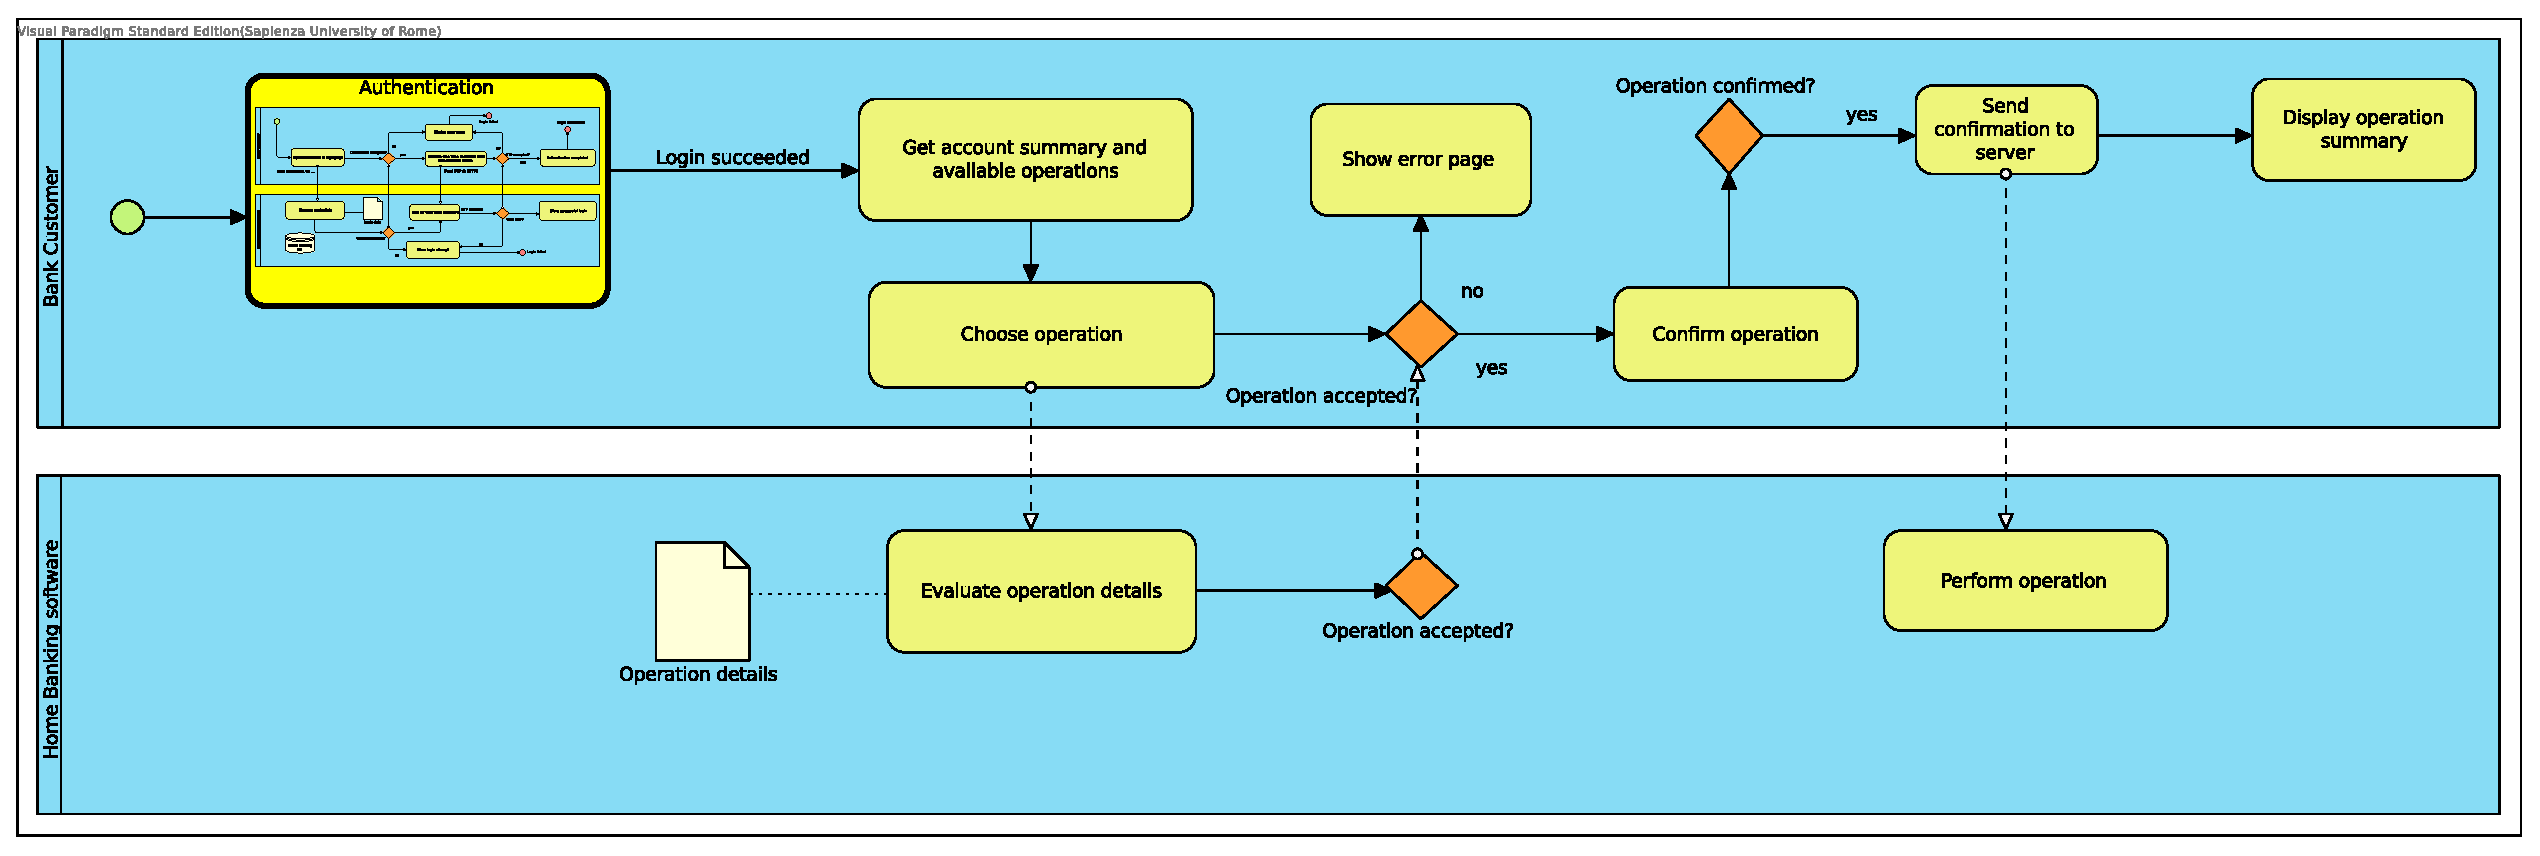
\includegraphics[width=\textheight, angle=90]{Images/Home_Banking_generic_action.eps}
	\caption{Business case: generica procedura di Home Banking effettuata da un utente del sistema.}
	\label{fig:business_case_generic_operation}
\end{figure*}

\end{document}
